\documentclass{beamer}
\usepackage{tikz,amsmath,hyperref,graphicx,stackrel,animate}
\usetikzlibrary{positioning,shadows,arrows,shapes,calc}
\newcommand{\argmax}{\operatornamewithlimits{argmax}}
\newcommand{\argmin}{\operatornamewithlimits{argmin}}
\mode<presentation>{\usetheme{Frankfurt}}
\DeclareMathOperator*{\softmax}{softmax}
\AtBeginSection[]
{
  \begin{frame}<beamer>
    \frametitle{Outline}
    \tableofcontents[currentsection,currentsubsection]
  \end{frame}
}
\title{Lecture 18: Backpropagation}
\author{Mark Hasegawa-Johnson}
\date{ECE 417: Multimedia Signal Processing, Fall 2021}  
\begin{document}

% Title
\begin{frame}
  \maketitle
\end{frame}

% Title
\begin{frame}
  \tableofcontents
\end{frame}


%%%%%%%%%%%%%%%%%%%%%%%%%%%%%%%%%%%%%%%%%%%%
\section[Review]{Review: Neural Network}
\setcounter{subsection}{1}

\begin{frame}
  \frametitle{Two-Layer Feedforward Neural Network}
  \begin{small}\begin{center}
  \tikzstyle{pre}=[<-,shorten <=1pt,>=stealth',semithick,draw=blue]
  \tikzstyle{post}=[->,shorten >=1pt,>=stealth',semithick,draw=blue]
  \begin{tikzpicture}[
      open/.style={circle,thick, draw=blue, text=black, align=left, text width=0.5cm}
    ]
    \node (x0) at (0,0.25) {$1$};
    \node[open] (x1) at (1,0) {$x_1$};
    \node[open] (x2) at (2,0) {$x_2$};
    \node (x3) at (2.75,0) {\ldots};
    \node[open] (xm0) at (3.5,0) {$x_{m_0}$};
    \node (input) at (6,0) {$\mathbf{a}_0=\mathbf{x}$ is the input vector};
    \node[open] (z11) at (1,1.3) {$z_{1,1}$} edge[pre](x0) edge[pre](x1) edge[pre](x2) edge[pre](xm0);
    \node[open] (z12) at (2,1.3) {$z_{1,2}$} edge[pre](x0) edge[pre](x1) edge[pre](x2) edge[pre](xm0);
    \node (z13) at (2.75,1.3) {\ldots};
    \node[open] (z1m1) at (3.5,1.3) {$z_{1,m_1}$} edge[pre](x0) edge[pre](x1) edge[pre](x2) edge[pre](xm0);
    \node (z1eq) at (6,1.3) {$\mathbf{z}_1=\mathbf{W}_1\mathbf{x}+\mathbf{b}_1$};
    \node (a10) at (0,2.7) {$1$};
    \node[open] (a11) at (1,2.45) {$a_{1,1}$} edge[pre](z11);
    \node[open] (a12) at (2,2.45) {$a_{1,2}$} edge[pre](z12);
    \node (a13) at (2.75,2.45) {\ldots};
    \node[open] (a1m1) at (3.5,2.45) {$a_{1,m_1}$} edge[pre](z1m1);
    \node (a1eq) at (6,2.45) {$\mathbf{a}_1=\mathbf{f}_1(\mathbf{z}_1)$};
    \node[open] (z21) at (1,3.75) {$z_{2,1}$} edge[pre](a10) edge[pre](a11) edge[pre](a12) edge[pre](a1m1);
    \node[open] (z22) at (2,3.75) {$z_{2,2}$} edge[pre](a10) edge[pre](a11) edge[pre](a12) edge[pre](a1m1);
    \node (z23) at (2.75,3.75) {\ldots};
    \node[open] (z2m2) at (3.5,3.75){$z_{2,m_2}$}edge[pre](a10) edge[pre](a11) edge[pre](a12) edge[pre](a1m1);
    \node (z2eq) at (6,3.75) {$\mathbf{z}_2=\mathbf{W}_2\mathbf{a}_1+\mathbf{b}_2$};
    \node[open] (a21) at (1,4.9) {$g_{1}$} edge[pre](z21);
    \node[open] (a22) at (2,4.9) {$g_{2}$} edge[pre](z22);
    \node (a23) at (2.75,4.9) {\ldots};
    \node[open] (a2m2) at (3.5,4.9) {$g_{m_2}$} edge[pre](z2m2);
    \node (z2eq) at (6,4.9) {$\mathbf{g}(\mathbf{x})=\mathbf{a}_2=\mathbf{f}_2(\mathbf{z}_2)$};
    \node (output) at (2.2,5.65) {${\mathcal{L}}=E\left[-\ln\Pr(\mathbf{y}|\mathbf{g}(\mathbf{x}))\right]$};
  \end{tikzpicture}
\end{center}
\end{small}
\end{frame}

\begin{frame}
  \frametitle{Review: Second Layer = Piece-Wise Approximation}

  The second layer of the network approximates $\hat{y}$ using a bias term $\vec{b}$,
  plus correction vectors $\vec{w}_j^{(2)}$, each scaled by its activation $h_j$:
  \[
  \hat{y} = \vec{b}^{(2)} + \sum_j \vec{w}_{j}^{(2)} h_j
  \]
  The activation, $h_j$, is a number between 0 and 1.  For example, we could
  use the logistic sigmoid function:
  \[
  h_k = \sigma\left(\xi_k^{(1)}\right)=\frac{1}{1+\exp(-\xi_k^{(1)})}\in\left(0,1\right)
  \]
  The logistic sigmoid is a differentiable approximation to a unit step function.
\end{frame}

\begin{frame}
  \frametitle{Review: First Layer = A Series of Decisions}

  The first layer of the network decides whether or not to ``turn on'' each of the
  $h_j$'s.  It does this by comparing $\vec{x}$ to a series of linear threshold vectors:
  \[
  h_k = \sigma\left(\bar{w}_k^{(1)}\vec{x}\right)\approx\begin{cases}
  1 & \bar{w}_k^{(1)}\vec{x} > 0\\
  0 & \bar{w}_k^{(1)}\vec{x} < 0
  \end{cases}
  \]
\end{frame}

%%%%%%%%%%%%%%%%%%%%%%%%%%%%%%%%%%%%%%%%%%%%%
\section[Learning]{Learning the Parameters of a Neural Network}
\setcounter{subsection}{1}

\begin{frame}
  \frametitle{How to train a neural network}
  \begin{enumerate}
  \item Find a {\bf training dataset} that contains $n$ examples showing the
    desired output, $\vec{y}_i$, that the NN should compute in
    response to input vector $\vec{x}_i$:
    \[
    {\mathcal D}=\left\{(\vec{x}_1,\vec{y}_1),\ldots,(\vec{x}_n,\vec{y}_n)\right\}
    \]
    \item Randomly {\bf initialize} $W^{(1)}$,
      $\vec{b}^{(1)}$, $W^{(2)}$, and $\vec{b}^{(2)}$.
    \item Perform {\bf forward propagation}: find out what the neural
      net computes as $\hat{y}_i$ for each $\vec{x}_i$.
    \item Define a {\bf loss function} that measures
      how badly $\hat{y}$ differs from $\vec{y}$.
    \item Perform {\bf back propagation} to find the derivative of the loss w.r.t.  $W^{(1)}$,
      $\vec{b}^{(1)}$, $W^{(2)}$, and $\vec{b}^{(2)}$.
    \item Perform {\bf gradient descent} to improve  $W^{(1)}$,
      $\vec{b}^{(1)}$, $W^{(2)}$, and $\vec{b}^{(2)}$.
    \item Repeat steps 3-6 until convergence.
  \end{enumerate}
\end{frame}

\begin{frame}
  \frametitle{Loss Function: How should $y$ be
    ``similar to'' $\hat{y}$?}
  \begin{block}{Minimum Mean Squared Error (MMSE)}
    \[
    W^*,b^*=\arg\min {\mathcal L} = \arg\min\frac{1}{2n}\sum_{i=1}^n
    \Vert\vec{y}_{i}-\hat{y}(\vec{x}_i)\Vert^2
    \]
  \end{block}
  \begin{block}{MMSE Solution: $\hat{y}\rightarrow E\left[\vec{y}|\vec{x}\right]$}
    If the training samples $(\vec{x}_i,\vec{y}_i)$ are i.i.d., then
    \[
    \lim_{n\rightarrow\infty}{\mathcal L} = \frac{1}{2}E\left[\Vert\vec{y}-\hat{y}\Vert^2\right]
    \]
    which is minimized by
    \[
    \hat{y}_{MMSE}(\vec{x})=E\left[\vec{y}|\vec{x}\right]
    \]
  \end{block}
\end{frame}

\begin{frame}
  \frametitle{Gradient Descent: How do we improve $W$ and $b$?}  Given
  some initial neural net parameter (called $u_{kj}$ in this figure),
  we want to find a better value of the same parameter.  We do that
  using gradient descent:
  \[
  u_{kj} \leftarrow u_{kj}-\eta\frac{d{\mathcal L}}{du_{kj}},
  \]
  where $\eta$ is a learning rate (some small constant, e.g., $\eta=0.02$ or so).
  \centerline{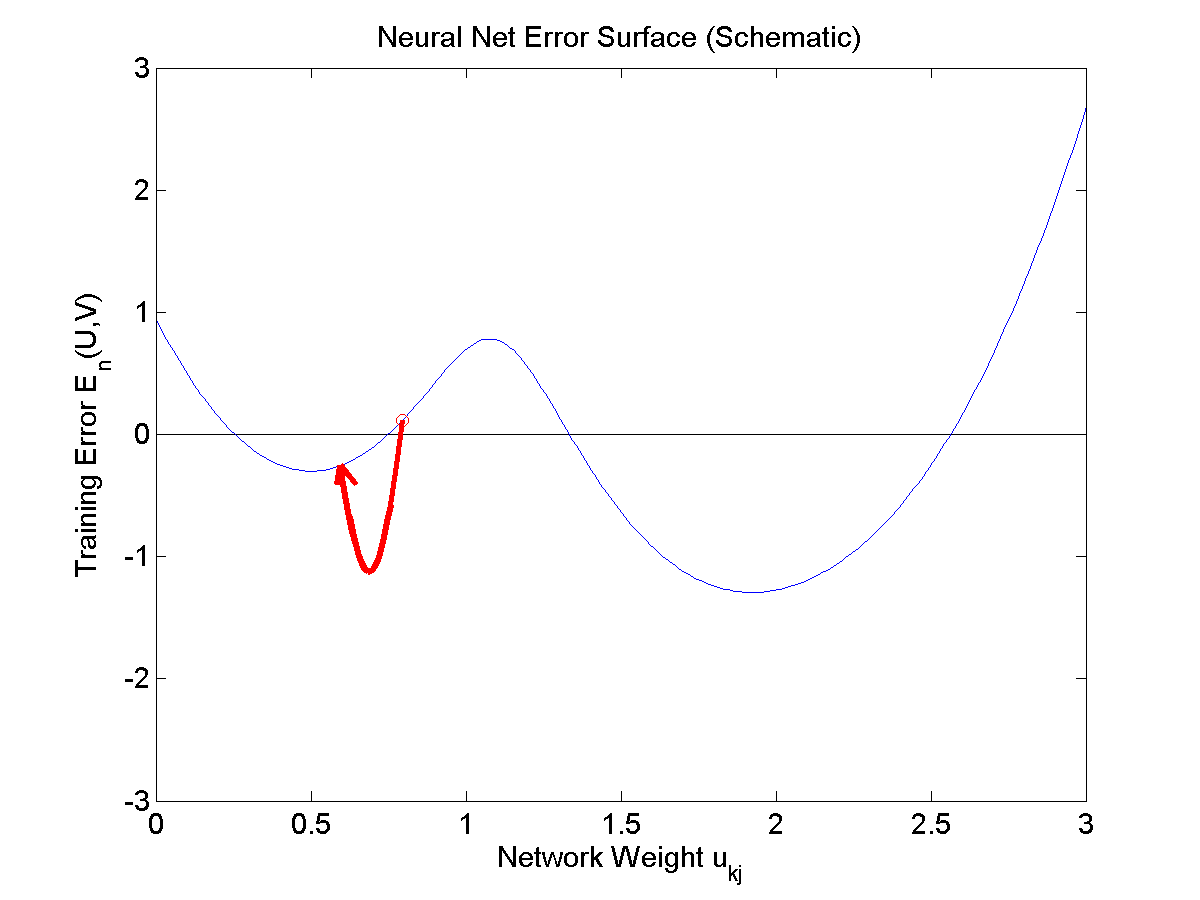
\includegraphics[width=2in]{figs/nn_errorsurf1.png}}
\end{frame}

\begin{frame}
\begin{block}{Gradient Descent = Local Optimization}
  Given an initial $W,b$, find new values of $W$, $b$ with lower error.
  \begin{align*}
    w_{kj}^{(1)} &\leftarrow w_{kj}^{(1)}-\eta\frac{d{\mathcal L}}{d w_{kj}^{(1)}}\\
    w_{kj}^{(2)} &\leftarrow w_{kj}^{(2)}-\eta\frac{d{\mathcal L}}{d w_{kj}^{(2)}}
  \end{align*}
\end{block}
\begin{block}{$\eta=$Learning Rate}
    \begin{itemize}
      \item If $\eta$ too large, gradient descent won't converge. If
        too small, convergence is slow.
      \item Second-order methods like Newton's method, L-BFGS and Adam choose an optimal $\eta$
        at each step, so they're MUCH faster.
    \end{itemize}
\end{block}
\end{frame}

%%%%%%%%%%%%%%%%%%%%%%%%%%%%%%%%%%%%%%%%%%%%%
\section[Gradient]{Definitions of Gradient, Partial Derivative, and Flow Graph}
\setcounter{subsection}{1}

\begin{frame}
  \frametitle{Digression: What is a Gradient?}

  The gradient of a scalar function, $f(\vec{w})$, with respect to
  the vector $\vec{w}$ can be usefully defined as
  \begin{displaymath}
    \nabla_{\vec{w}} f=\left[\begin{array}{c}
        \frac{\partial f}{\partial w_{1}}\\
        \frac{\partial f}{\partial w_{2}}\\
        \vdots\\
        \frac{\partial f}{\partial w_{N}}
      \end{array}\right],~~\mbox{where}~~
    \vec{w}=\left[\begin{array}{cccc}
        w_{1}\\
        w_{2}\\
        \vdots\\
        w_{N}
      \end{array}\right].
  \end{displaymath}
  Here the {\bf partial derivative} sign, $\partial$, means ``the
  derivative while all other elements of $\vec{w}$ are held
  constant.''
\end{frame}

\begin{frame}
  \frametitle{Digression: Total Derivative vs.~Partial Derivative}
  
  \begin{itemize}
  \item The notation $\frac{d{\mathcal L}}{dw_{kj}^{(2)}}$ means
    ``the total derivative of ${\mathcal L}$ with respect to
    $w_{kj}^{(2)}$.'' It implies that we have to add up several
    different ways in which ${\mathcal L}$ depends on
    $w_{kj}^{(2)}$, for example,
    \begin{align*}
      \frac{d{\mathcal L}}{dw_{kj}^{(2)}} &=
      \sum_{i=1}^n
      \left(\frac{d{\mathcal L}}{d\hat{y}_{ki}}\right)
      \left(\frac{\partial\hat{y}_{ki}}{\partial w_{kj}^{(2)}}\right)
    \end{align*}
  \item The notation $\frac{\partial{\mathcal
      L}}{\partial\hat{y}_{ki}}$ means ``partial derivative.''  It
    means ``hold other variables constant while calculating this
    derivative.''
  \item The next obvious question to ask is: {\bf which} other variables
    should I hold constant?
  \end{itemize}
\end{frame}

\begin{frame}
  \frametitle{Flow Graph}

  A signal flow graph shows the flow of computations in a system.  For
  example, the following graph shows that $y$ is a function of
  $\{g,h\}$, $g$ is a function of $\{x,z\}$, and $h$ is a
  function of $\{x,z\}$:

  \begin{center}
    \tikzstyle{pre}=[<-,shorten <=1pt,>=stealth',semithick,draw=blue]
    \tikzstyle{post}=[->,shorten >=1pt,>=stealth',semithick,draw=blue]
    \begin{tikzpicture}[
        hoop/.style={circle,thick, draw=blue, text=black, fill=orange!35!white, text centered, text width=0.25cm},
        open/.style={circle,thick, draw=blue, text=black, text centered, text width=0.25cm}
      ]
      \node[open] (x) at (0,-1) {$x$};
      \node[open] (z) at (0,1) {$z$};
      \node[open] (g) at (2,-1) {$g$} edge[pre](x) edge[pre](z);
      \node[open] (h) at (2,1) {$h$} edge[pre](x) edge[pre](z);
      \node[open] (y) at (4,0) {$y$} edge[pre](g) edge[pre](h);
    \end{tikzpicture}
  \end{center}
\end{frame}

\begin{frame}
  \frametitle{The Total Derivative Rule}

  The {\bf total derivative rule} says that the derivative of the
  output with respect to any one input can be computed as the sum of
  partial times total, summed across all paths from input to output:

  \begin{displaymath}
    \frac{\partial y}{\partial x} =
    \left(\frac{\partial y}{\partial g}\right)\left(\frac{dg}{dx}\right) +
    \left(\frac{\partial y}{\partial h}\right)\left(\frac{dh}{dx}\right)
  \end{displaymath}

  \begin{center}
    \tikzstyle{pre}=[<-,shorten <=1pt,>=stealth',semithick,draw=blue]
    \tikzstyle{post}=[->,shorten >=1pt,>=stealth',semithick,draw=blue]
    \begin{tikzpicture}[
        hoop/.style={circle,thick, draw=blue, text=black, fill=orange!35!white, text centered, text width=0.25cm},
        open/.style={circle,thick, draw=blue, text=black, text centered, text width=0.25cm}
      ]
      \node[open] (x) at (0,-1) {$x$};
      \node[open] (z) at (0,1) {$z$};
      \node[open] (g) at (2,-1) {$g$} edge[pre](x) edge[pre](z);
      \node[open] (h) at (2,1) {$h$} edge[pre](x) edge[pre](z);
      \node[open] (y) at (4,0) {$y$} edge[pre](g) edge[pre](h);
    \end{tikzpicture}
  \end{center}
\end{frame}

\begin{frame}
  \frametitle{Partial with respect to What?}

  The difference between {\bf partial derivative} and {\bf total
    derivative} only makes sense in light of the total derivative
  rule. For example, in this equation 
  \begin{displaymath}
    \frac{\partial y}{\partial x} =
    \left(\frac{\partial y}{\partial g}\right)\left(\frac{dg}{dx}\right) +
    \left(\frac{\partial y}{\partial h}\right)\left(\frac{dh}{dx}\right)
  \end{displaymath}
  \begin{itemize}
  \item The symbol $\frac{\partial y}{\partial g}$ means ``the
    derivative of $y$ with respect to $g$ while holding $h$ constant.''
  \item The symbol $\frac{dg}{dx}$ means ``the derivative of $g$ with
    respect to $x$, {\bf without} holding $h$ constant.''
  \item For today's lecture, the difference between partial and total
    derivative doesn't matter much, because it doesn't matter whether
    you hold $h$ constant or not.  When we get into recurrent neural
    networks, later, such things will start to matter, so we'll
    discuss this point again at that time.
  \end{itemize}
\end{frame}

%%%%%%%%%%%%%%%%%%%%%%%%%%%%%%%%%%%%%%%%%%%%%
\section[Back-Propagation]{Back-Propagation}
\setcounter{subsection}{1}

\begin{frame}
  \frametitle{Computing the Gradient: Notation}
  \begin{itemize}
  \item $\vec{x}_i=[x_{1i},\ldots,x_{Di}]^T$ is the $i^{\textrm{th}}$ input vector.
  \item $\vec{y}_i=[y_{1i},\ldots,y_{Ki}]^T$ is the $i^{\textrm{th}}$ target vector (desired output).
  \item $\hat{y}_i=[\hat{y}_{1i},\ldots,\hat{y}_{Ki}]^T$ is the
    $i^{\textrm{th}}$ hypothesis vector (computed output).
  \item $\vec\xi_i^{(l)}=[\xi_{1i}^{(l)},\ldots,\xi_{Ni}^{(l)}]^T$ is the
    excitation vector after the $l^{\textrm{th}}$ layer, in response
    to the $i^{\textrm{th}}$ input.
  \item $\vec{h}_i=[h_{1i},\ldots,h_{Ni}]^T$ is the hidden nodes
    activation vector in response to the $i^{\textrm{th}}$ input. (No
     superscript necessary if there's only one hidden layer).
  \item The weight matrix for the $l^{\textrm{th}}$ layer is
    \[
    W^{(l)}=\left[\vec{w}_1^{(l)},\ldots,\vec{w}_j^{(l)},\ldots\right]=
    \left[\begin{array}{cccc}
        w_{11}^{(l)}&\cdots&w_{1j}^{(l)}&\cdots\\
        \vdots &\ddots&\vdots&\ddots\\
        w_{k1}^{(l)}&\cdots&w_{kj}^{(l)}&\cdots\\
        \vdots &\ddots&\vdots&\ddots
      \end{array}\right]
    \]
  \end{itemize}
\end{frame}
      
\begin{frame}
  \frametitle{Two-Layer Feedforward Neural Network}
  \begin{small}\begin{center}
  \tikzstyle{pre}=[<-,shorten <=1pt,>=stealth',semithick,draw=blue]
  \tikzstyle{post}=[->,shorten >=1pt,>=stealth',semithick,draw=blue]
  \begin{tikzpicture}[
      open/.style={circle,thick, draw=blue, text=black, align=left, text width=0.5cm}
    ]
    \node (x0) at (0,0.25) {$1$};
    \node[open] (x1) at (1,0) {$x_1$};
    \node[open] (x2) at (2,0) {$x_2$};
    \node (x3) at (2.75,0) {\ldots};
    \node[open] (xm0) at (3.5,0) {$x_{m_0}$};
    \node (input) at (6,0) {$\mathbf{a}_0=\mathbf{x}$ is the input vector};
    \node[open] (z11) at (1,1.3) {$z_{1,1}$} edge[pre](x0) edge[pre](x1) edge[pre](x2) edge[pre](xm0);
    \node[open] (z12) at (2,1.3) {$z_{1,2}$} edge[pre](x0) edge[pre](x1) edge[pre](x2) edge[pre](xm0);
    \node (z13) at (2.75,1.3) {\ldots};
    \node[open] (z1m1) at (3.5,1.3) {$z_{1,m_1}$} edge[pre](x0) edge[pre](x1) edge[pre](x2) edge[pre](xm0);
    \node (z1eq) at (6,1.3) {$\mathbf{z}_1=\mathbf{W}_1\mathbf{x}+\mathbf{b}_1$};
    \node (a10) at (0,2.7) {$1$};
    \node[open] (a11) at (1,2.45) {$a_{1,1}$} edge[pre](z11);
    \node[open] (a12) at (2,2.45) {$a_{1,2}$} edge[pre](z12);
    \node (a13) at (2.75,2.45) {\ldots};
    \node[open] (a1m1) at (3.5,2.45) {$a_{1,m_1}$} edge[pre](z1m1);
    \node (a1eq) at (6,2.45) {$\mathbf{a}_1=\mathbf{f}_1(\mathbf{z}_1)$};
    \node[open] (z21) at (1,3.75) {$z_{2,1}$} edge[pre](a10) edge[pre](a11) edge[pre](a12) edge[pre](a1m1);
    \node[open] (z22) at (2,3.75) {$z_{2,2}$} edge[pre](a10) edge[pre](a11) edge[pre](a12) edge[pre](a1m1);
    \node (z23) at (2.75,3.75) {\ldots};
    \node[open] (z2m2) at (3.5,3.75){$z_{2,m_2}$}edge[pre](a10) edge[pre](a11) edge[pre](a12) edge[pre](a1m1);
    \node (z2eq) at (6,3.75) {$\mathbf{z}_2=\mathbf{W}_2\mathbf{a}_1+\mathbf{b}_2$};
    \node[open] (a21) at (1,4.9) {$g_{1}$} edge[pre](z21);
    \node[open] (a22) at (2,4.9) {$g_{2}$} edge[pre](z22);
    \node (a23) at (2.75,4.9) {\ldots};
    \node[open] (a2m2) at (3.5,4.9) {$g_{m_2}$} edge[pre](z2m2);
    \node (z2eq) at (6,4.9) {$\mathbf{g}(\mathbf{x})=\mathbf{a}_2=\mathbf{f}_2(\mathbf{z}_2)$};
    \node (output) at (2.2,5.65) {${\mathcal{L}}=E\left[-\ln\Pr(\mathbf{y}|\mathbf{g}(\mathbf{x}))\right]$};
  \end{tikzpicture}
\end{center}
\end{small}
\end{frame}

\begin{frame}
  \frametitle{Two-Layer Feedforward Neural Network}
  \begin{small}      \begin{center}
        \tikzstyle{pre}=[<-,shorten <=1pt,>=stealth',semithick,draw=blue]
        \tikzstyle{post}=[->,shorten >=1pt,>=stealth',semithick,draw=blue]
        \begin{tikzpicture}[
            hoop/.style={circle,thick, draw=blue, text=black, fill=orange!35!white, text centered, text width=0.25cm},
            open/.style={circle,thick, draw=blue, text=black, text centered, text width=0.25cm}
          ]
          \node (x0) at (0,0) {$1$};
          \node[open] (x1) at (1,0) {$x_1$};
          \node[open] (x2) at (2,0) {$x_2$};
          \node (x3) at (3,0) {\ldots};
          \node[open] (xp) at (4,0) {$x_D$};
          \node (input) at (7,0) {$\vec{x}$ is the input vector};
          \node (e1sum) at (7,0.75) {$\vec\xi^{(1)} = \vec{b}^{(1)}+W^{(1)}\vec{x}$};
          %\node (e1vec) at (9,0.75) {$\vec{e}^{(1)}=W^{(1)}\vec{x}+\vec{b}^{(1)}$};
          \node (h0) at (0,1.5) {$1$};
          \node[hoop] (h1) at (1,1.5) {$h_1$} edge[pre](x0) edge[pre](x1) edge[pre](xp);
          \node[hoop] (h2) at (2,1.5) {$h_2$} edge[pre](x0) edge[pre](x1) edge[pre](xp);
          \node (y3) at (3,1.5) {\ldots};
          \node[hoop] (hq) at (4,1.5) {$h_N$} edge[pre](x0) edge[pre](x1) edge[pre](xp);
          \node (hsum) at (7,1.5) {$\vec{h}=\sigma(\vec\xi^{(1)})$};
          %\node (hvec) at (9,1.5) {$\vec{h}=f(\vec{e}^{(1)})$};
          \node (e2sum) at (7,2.25) {$\vec\xi^{(2)}=\vec{b}^{(2)}+W^{(2)}\vec{h}$};
          %\node (e2vec) at (9,2.25) {$\vec{e}^{(2)}=W^{(2)}\vec{h}+\vec{b}^{(2)}$};
          \node[hoop] (y1) at (1,3) {$\hat{y}_1$} edge[pre](h0) edge[pre](h1) edge[pre](hq);
          \node[hoop] (y2) at (2,3) {$\hat{y}_2$} edge[pre](h0) edge[pre](h1) edge[pre](hq);
          \node (y3) at (3,3) {\ldots};
          \node[hoop] (yr) at (4,3) {$\hat{y}_K$} edge[pre](h0) edge[pre](h1) edge[pre](hq);
          \node (ysum) at (7,3) {$\hat{y}=\vec\xi^{(2)}$};
          %\node (yvec) at (9,3) {$\hat{y}=\vec{e}^{(2)}$};
          \node (zeta1) at (1,3.75) {} edge[pre](y1);
          \node (zeta2) at (2,3.75) {} edge[pre](y2);
          \node (zetar) at (4,3.75) {} edge[pre](yr);
          \node (output) at (2.5,4) {$\hat{y}=f(\vec{x},W^{(1)},\vec{b}^{(1)},W^{(2)},\vec{b}^{(2)})$};
        \end{tikzpicture}
      \end{center}
\end{small}
\end{frame}

\begin{frame}
  \frametitle{Back-Propagation}

  Back-propagation just works backward through this network, calculating
  the derivative of ${\mathcal L}$ with respect to $\hat{y}$, then $\vec\xi^{(2)}$, then
  $\vec{h}$, then $\vec\xi^{(1)}$:
  \begin{small}      \begin{center}
        \tikzstyle{pre}=[<-,shorten <=1pt,>=stealth',semithick,draw=blue]
        \tikzstyle{post}=[->,shorten >=1pt,>=stealth',semithick,draw=blue]
        \begin{tikzpicture}[
            hoop/.style={circle,thick, draw=blue, text=black, fill=orange!35!white, text centered, text width=0.25cm},
            open/.style={circle,thick, draw=blue, text=black, text centered, text width=0.25cm}
          ]
          \node (x0) at (0,0) {$1$};
          \node[open] (x1) at (1,0) {$x_1$};
          \node[open] (x2) at (2,0) {$x_2$};
          \node (x3) at (3,0) {\ldots};
          \node[open] (xp) at (4,0) {$x_D$};
          \node (input) at (7,0) {$\vec{x}$ is the input vector};
          \node (e1sum) at (7,0.75) {$\vec\xi^{(1)} = \vec{b}^{(1)}+W^{(1)}\vec{x}$};
          %\node (e1vec) at (9,0.75) {$\vec{e}^{(1)}=W^{(1)}\vec{x}+\vec{b}^{(1)}$};
          \node (h0) at (0,1.5) {$1$};
          \node[hoop] (h1) at (1,1.5) {$h_1$} edge[pre](x0) edge[pre](x1) edge[pre](xp);
          \node[hoop] (h2) at (2,1.5) {$h_2$} edge[pre](x0) edge[pre](x1) edge[pre](xp);
          \node (y3) at (3,1.5) {\ldots};
          \node[hoop] (hq) at (4,1.5) {$h_N$} edge[pre](x0) edge[pre](x1) edge[pre](xp);
          \node (hsum) at (7,1.5) {$\vec{h}=\sigma(\vec\xi^{(1)})$};
          %\node (hvec) at (9,1.5) {$\vec{h}=f(\vec{e}^{(1)})$};
          \node (e2sum) at (7,2.25) {$\vec\xi^{(2)}=\vec{b}^{(2)}+W^{(2)}\vec{h}$};
          %\node (e2vec) at (9,2.25) {$\vec{e}^{(2)}=W^{(2)}\vec{h}+\vec{b}^{(2)}$};
          \node[hoop] (y1) at (1,3) {$\hat{y}_1$} edge[pre](h0) edge[pre](h1) edge[pre](hq);
          \node[hoop] (y2) at (2,3) {$\hat{y}_2$} edge[pre](h0) edge[pre](h1) edge[pre](hq);
          \node (y3) at (3,3) {\ldots};
          \node[hoop] (yr) at (4,3) {$\hat{y}_K$} edge[pre](h0) edge[pre](h1) edge[pre](hq);
          \node (ysum) at (7,3) {$\hat{y}=\vec\xi^{(2)}$};
          %\node (yvec) at (9,3) {$\hat{y}=\vec{e}^{(2)}$};
          \node (zeta1) at (1,3.75) {} edge[pre](y1);
          \node (zeta2) at (2,3.75) {} edge[pre](y2);
          \node (zetar) at (4,3.75) {} edge[pre](yr);
          \node (output) at (2.5,4) {$\hat{y}=f(\vec{x},W^{(1)},\vec{b}^{(1)},W^{(2)},\vec{b}^{(2)})$};
        \end{tikzpicture}
      \end{center}
\end{small}
\end{frame}

\begin{frame}
  \frametitle{Back-Propagation: Derivative w.r.t Output-Layer Activations}

  Remember that the loss function  is mean-squared error:
  \begin{align*}
    {\mathcal L}&=\frac{1}{2n}\sum_{i=1}^n \Vert\vec{y}_i-\hat{y}_i\Vert^2\\
    &=\frac{1}{2n}\sum_{i=1}^n\sum_{k=1}^K (\vec{y}_{i,k}-\hat{y}_{i,k})^2
  \end{align*}
  So:
  \begin{align*}
    \frac{\partial\mathcal L}{\partial \hat{y}_{i,k}} &= \frac{1}{n}(\hat{y}_{i,k}-y_{i,k})
  \end{align*}
\end{frame}
  
\begin{frame}
  \frametitle{Back-Propagation: Derivative w.r.t Output-Layer Excitations}

  In our network, the output layer is linear, so
  \begin{align*}
    \hat{y}_{i,k} = \xi_{i,k}^{(2)}
  \end{align*}
  Therefore:
  \begin{align*}
    \frac{\partial\mathcal L}{\partial \xi_{i,k}^{(2)}} &= \frac{1}{n}(\hat{y}_{i,k}-y_{i,k})
  \end{align*}
\end{frame}
  
\begin{frame}
  \frametitle{The back-prop deltas: derivative w.r.t. excitations}

  In order to keep going systematically, it's useful to define a {\bf
    back-propagation partial derivative}:
  \begin{align*}
    \delta_{i,k}^{(2)}\equiv\frac{\partial\mathcal L}{\partial \xi_{i,k}^{(2)}}
  \end{align*}
  These deltas are sometimes called the {\bf excitation gradients}:
  \begin{align*}
    \vec\delta_i^{(2)} = \nabla_{\vec\xi_i^{(2)}}{\mathcal L}
  \end{align*}
\end{frame}

\begin{frame}
  \frametitle{Back-Propagation: Derivative w.r.t Hidden-Layer Activations}

  The mapping from {\bf hidden-layer activations} to {\bf output-layer excitations} is 
  \begin{align*}
    \xi_{i,k}^{(2)} &=b_k^{(2)} + \sum_{j=1}^Nw_{k,j}^{(2)} h_{i,j}
  \end{align*}
  Notice that the loss, ${\mathcal L}$, depends on $h_{i,j}$ via all
  of the different paths through all of the different
  $\xi_{i,k}^{(2)}$ output excitations.  The {\bf total derivative
    rule} therefore gives us:
  \begin{align*}
    \frac{\partial\mathcal L}{\partial h_{i,j}} &=
    \sum_{k=1}^K\left(\frac{\partial\mathcal L}{\partial\xi_{i,k}^{(2)}}\right)
    \left(\frac{\partial\xi_{i,k}^{(2)}}{\partial h_{i,j}}\right)\\
    &=    \sum_{k=1}^K\delta_{i,k}^{(2)} w_{k,j}^{(2)}
  \end{align*}
\end{frame}

\begin{frame}
  \frametitle{Back-Propagation: Derivative w.r.t Hidden-Layer Activations}

  The mapping from {\bf hidden-layer activations} to {\bf output-layer excitations} is 
  \begin{align*}
    \vec\xi_i^{(2)} &=\vec{b}^{(2)} + W^{(2)}\vec{h}_i
  \end{align*}
  Notice that the loss, ${\mathcal L}$, depends on $h_{j,i}$ via all
  of the different paths through all of the different
  $\xi_{k,i}^{(2)}$ output excitations.  The {\bf total derivative
    rule} therefore gives us the following surprising rule:
  \begin{align*}
    \nabla_{\vec{h}_i}{\mathcal L}     &= W^{(2),T} \nabla_{\vec\xi_i^{(2)}}{\mathcal L}\\
    &= W^{(2),T} \vec\delta_i^{(2)}
  \end{align*}
\end{frame}

\begin{frame}
  \frametitle{Back-Propagation: Derivative w.r.t Hidden-Layer Excitations}

  The mapping from {\bf hidden-layer excitations} to {\bf hidden-layer activations} is
  much simpler:
  \begin{align*}
    h_{i,j} = \sigma(\xi_{i,j}^{(1)})
  \end{align*}
  So
  \begin{align*}
    \frac{\partial\mathcal L}{\partial \xi_{i,j}^{(1)}} &=
    \left(\frac{\partial\mathcal L}{\partial h_{i,j}}\right)
    \left(\frac{\partial h_{i,j}}{\partial \xi_{i,j}^{(1)}}\right)\\
    &=
    \left(\sum_{k=1}^K w_{k,j}^{(2)}\delta_{i,j}^{(2)}\right)
    \left(\dot\sigma\left(\xi_{i,j}^{(1)}\right)\right)
  \end{align*}
  where $\dot\sigma(\cdot)$, the derivative of the scalar nonlinearity
  $\sigma(\cdot)$, is something you can calculate in advance, and store.
\end{frame}

\begin{frame}
  \frametitle{Back-Propagation: Derivative w.r.t Hidden-Layer Excitations}

  We can define {\bf excitation gradients} at  the hidden layer to be
  \begin{align*}
    \vec\delta_i^{(1)} = \nabla_{\vec\xi_i^{(1)}}{\mathcal L}
  \end{align*}

  Putting together the last two steps, we have that
  \begin{align*}
    \vec\delta_i^{(1)} = \left(W^{(2),T}\vec\delta_i^{(2)}\right) \odot
    \dot\sigma\left(\xi_i^{(1)}\right)
  \end{align*}
  where $\odot$ means Hadamard product (element-wise multiplication of the two vectors).
\end{frame}

%%%%%%%%%%%%%%%%%%%%%%%%%%%%%%%%%%%%%%%%%%%%%
\section[Derivatives]{Computing the Weight Derivatives}
\setcounter{subsection}{1}


\begin{frame}
  \frametitle{Computing the Derivative}
  OK, let's compute the derivative of ${\mathcal L}$ with respect to the $W^{(2)}$
  matrix.  Remember that $W^{(2)}$ enters the neural net computation as
  $\xi_{ki}^{(2)}=\sum_k w_{kj}^{(2)}h_{ji}$.  So\ldots
  \begin{align*}
    \frac{d{\mathcal L}}{dw_{k,j}^{(2)}} &=
    \sum_{i=1}^n
    \left(\frac{d{\mathcal L}}{d\xi_{i,k}^{(2)}}\right)
    \left(\frac{\partial \xi_{i,k}^{(2)}}{\partial w_{k,j}^{(2)}}\right)\\
    &= \sum_{i=1}^n \delta^{(2)}_{k,i}h_{i,j}
  \end{align*}
  If we define the gradient of a matrix as a matrix of partial
  derivatives, we can write:
  \begin{align*}
    \nabla_{W^{(2)}}{\mathcal L} = \sum_{i=1}^n \vec\delta_i^{(2)}\vec{h}_i^T
    = \sum_{i=1}^n
    \left[\begin{array}{c}\vdots\\\frac{\partial\mathcal L}{\partial\xi_{i,k}^{(2)}}\\\vdots
      \end{array}\right]
    \left[\cdots, h_{i,j}, \cdots\right]
  \end{align*}
\end{frame}

\begin{frame}
  \begin{small}\begin{center}
  \tikzstyle{pre}=[<-,shorten <=1pt,>=stealth',semithick,draw=blue]
  \tikzstyle{post}=[->,shorten >=1pt,>=stealth',semithick,draw=blue]
  \begin{tikzpicture}[
      open/.style={circle,thick, draw=blue, text=black, align=left, text width=0.5cm}
    ]
    \node (x0) at (0,0.25) {$1$};
    \node[open] (x1) at (1,0) {$x_1$};
    \node[open] (x2) at (2,0) {$x_2$};
    \node (x3) at (2.75,0) {\ldots};
    \node[open] (xm0) at (3.5,0) {$x_{m_0}$};
    \node (input) at (6,0) {$\mathbf{a}_0=\mathbf{x}$ is the input vector};
    \node[open] (z11) at (1,1.3) {$z_{1,1}$} edge[pre](x0) edge[pre](x1) edge[pre](x2) edge[pre](xm0);
    \node[open] (z12) at (2,1.3) {$z_{1,2}$} edge[pre](x0) edge[pre](x1) edge[pre](x2) edge[pre](xm0);
    \node (z13) at (2.75,1.3) {\ldots};
    \node[open] (z1m1) at (3.5,1.3) {$z_{1,m_1}$} edge[pre](x0) edge[pre](x1) edge[pre](x2) edge[pre](xm0);
    \node (z1eq) at (6,1.3) {$\mathbf{z}_1=\mathbf{W}_1\mathbf{x}+\mathbf{b}_1$};
    \node (a10) at (0,2.7) {$1$};
    \node[open] (a11) at (1,2.45) {$a_{1,1}$} edge[pre](z11);
    \node[open] (a12) at (2,2.45) {$a_{1,2}$} edge[pre](z12);
    \node (a13) at (2.75,2.45) {\ldots};
    \node[open] (a1m1) at (3.5,2.45) {$a_{1,m_1}$} edge[pre](z1m1);
    \node (a1eq) at (6,2.45) {$\mathbf{a}_1=\mathbf{f}_1(\mathbf{z}_1)$};
    \node[open] (z21) at (1,3.75) {$z_{2,1}$} edge[pre](a10) edge[pre](a11) edge[pre](a12) edge[pre](a1m1);
    \node[open] (z22) at (2,3.75) {$z_{2,2}$} edge[pre](a10) edge[pre](a11) edge[pre](a12) edge[pre](a1m1);
    \node (z23) at (2.75,3.75) {\ldots};
    \node[open] (z2m2) at (3.5,3.75){$z_{2,m_2}$}edge[pre](a10) edge[pre](a11) edge[pre](a12) edge[pre](a1m1);
    \node (z2eq) at (6,3.75) {$\mathbf{z}_2=\mathbf{W}_2\mathbf{a}_1+\mathbf{b}_2$};
    \node[open] (a21) at (1,4.9) {$g_{1}$} edge[pre](z21);
    \node[open] (a22) at (2,4.9) {$g_{2}$} edge[pre](z22);
    \node (a23) at (2.75,4.9) {\ldots};
    \node[open] (a2m2) at (3.5,4.9) {$g_{m_2}$} edge[pre](z2m2);
    \node (z2eq) at (6,4.9) {$\mathbf{g}(\mathbf{x})=\mathbf{a}_2=\mathbf{f}_2(\mathbf{z}_2)$};
    \node (output) at (2.2,5.65) {${\mathcal{L}}=E\left[-\ln\Pr(\mathbf{y}|\mathbf{g}(\mathbf{x}))\right]$};
  \end{tikzpicture}
\end{center}
\end{small}
  \begin{block}{Back-Propagating to the First Layer}    
    \[
    \frac{d{\mathcal L}}{d w_{k,j}^{(1)}} =
    \sum_{i=1}^n
    \left(\frac{d{\mathcal L}}{d\xi_{i,k}^{(1)}}\right)
    \left(\frac{\partial \xi_{i,k}^{(1)}}{\partial w_{k,j}^{(1)}}\right)
    = \sum_{i=1}^n \delta^{(1)}_{i,k}x_{i,j}
    \]
  \end{block}
\end{frame}

\begin{frame}
  \begin{small}\begin{center}
  \tikzstyle{pre}=[<-,shorten <=1pt,>=stealth',semithick,draw=blue]
  \tikzstyle{post}=[->,shorten >=1pt,>=stealth',semithick,draw=blue]
  \begin{tikzpicture}[
      open/.style={circle,thick, draw=blue, text=black, align=left, text width=0.5cm}
    ]
    \node (x0) at (0,0.25) {$1$};
    \node[open] (x1) at (1,0) {$x_1$};
    \node[open] (x2) at (2,0) {$x_2$};
    \node (x3) at (2.75,0) {\ldots};
    \node[open] (xm0) at (3.5,0) {$x_{m_0}$};
    \node (input) at (6,0) {$\mathbf{a}_0=\mathbf{x}$ is the input vector};
    \node[open] (z11) at (1,1.3) {$z_{1,1}$} edge[pre](x0) edge[pre](x1) edge[pre](x2) edge[pre](xm0);
    \node[open] (z12) at (2,1.3) {$z_{1,2}$} edge[pre](x0) edge[pre](x1) edge[pre](x2) edge[pre](xm0);
    \node (z13) at (2.75,1.3) {\ldots};
    \node[open] (z1m1) at (3.5,1.3) {$z_{1,m_1}$} edge[pre](x0) edge[pre](x1) edge[pre](x2) edge[pre](xm0);
    \node (z1eq) at (6,1.3) {$\mathbf{z}_1=\mathbf{W}_1\mathbf{x}+\mathbf{b}_1$};
    \node (a10) at (0,2.7) {$1$};
    \node[open] (a11) at (1,2.45) {$a_{1,1}$} edge[pre](z11);
    \node[open] (a12) at (2,2.45) {$a_{1,2}$} edge[pre](z12);
    \node (a13) at (2.75,2.45) {\ldots};
    \node[open] (a1m1) at (3.5,2.45) {$a_{1,m_1}$} edge[pre](z1m1);
    \node (a1eq) at (6,2.45) {$\mathbf{a}_1=\mathbf{f}_1(\mathbf{z}_1)$};
    \node[open] (z21) at (1,3.75) {$z_{2,1}$} edge[pre](a10) edge[pre](a11) edge[pre](a12) edge[pre](a1m1);
    \node[open] (z22) at (2,3.75) {$z_{2,2}$} edge[pre](a10) edge[pre](a11) edge[pre](a12) edge[pre](a1m1);
    \node (z23) at (2.75,3.75) {\ldots};
    \node[open] (z2m2) at (3.5,3.75){$z_{2,m_2}$}edge[pre](a10) edge[pre](a11) edge[pre](a12) edge[pre](a1m1);
    \node (z2eq) at (6,3.75) {$\mathbf{z}_2=\mathbf{W}_2\mathbf{a}_1+\mathbf{b}_2$};
    \node[open] (a21) at (1,4.9) {$g_{1}$} edge[pre](z21);
    \node[open] (a22) at (2,4.9) {$g_{2}$} edge[pre](z22);
    \node (a23) at (2.75,4.9) {\ldots};
    \node[open] (a2m2) at (3.5,4.9) {$g_{m_2}$} edge[pre](z2m2);
    \node (z2eq) at (6,4.9) {$\mathbf{g}(\mathbf{x})=\mathbf{a}_2=\mathbf{f}_2(\mathbf{z}_2)$};
    \node (output) at (2.2,5.65) {${\mathcal{L}}=E\left[-\ln\Pr(\mathbf{y}|\mathbf{g}(\mathbf{x}))\right]$};
  \end{tikzpicture}
\end{center}
\end{small}
  \begin{block}{Back-Propagating to the First Layer}    
    \[
    \nabla_{W^{(1)}}{\mathcal L} = 
    \sum_{i=1}^n\vec\delta_i^{(1)}\vec{x}_i^T
    \]
  \end{block}
\end{frame}

\begin{frame}
  \begin{block}{The Back-Propagation Algorithm}
    \[
    W^{(2)}\leftarrow W^{(2)}-\eta\nabla_{W^{(2)}}{\mathcal L},~~~~~
    W^{(1)}\leftarrow W^{(1)}-\eta\nabla_{W^{(1)}}{\mathcal L}
    \]
    \[
    \nabla_{W^{(2)}}{\mathcal L}=\sum_{i=1}^n \vec\delta^{(2)}_i\vec{h}_i^T,~~~~~
    \nabla_{W^{(1)}}{\mathcal L}=\sum_{i=1}^n\vec\delta^{(1)}_i\vec{x}_i^T
    \]
    \[
    \delta^{(2)}_{i,k}=\frac{1}{n} (\hat{y}_{ki}-y_{ki}),~~~~~
    \delta^{(1)}_{i,k}=\sum_{\ell=1}^K \delta^{(2)}_{i,\ell}w_{\ell, k}^{(2)}\dot\sigma(\xi_{i,k}^{(1)})
    \]
    \[
    \vec\delta^{(2)}_i=\frac{1}{n}\left(\hat{y}_i-\vec{y}_i\right),~~~~~
    \vec\delta^{(1)}_i=\left(W^{(2),T}\vec\delta^{(2)}_i\right)\odot \dot\sigma(\vec\xi_i^{(1)})
    \]
    \ldots where $\odot$ means element-wise multiplication of two
    vectors; $\dot\sigma(\vec\xi)$ is the element-wise
    derivative of $\sigma(\vec\xi)$.
  \end{block}
\end{frame}

%%%%%%%%%%%%%%%%%%%%%%%%%%%%%%%%%%%%%%%%%%%%%%%%%%%%%%%%%%%%%%%
\section[Backprop Example]{Backprop Example: Semicircle $\rightarrow$ Parabola}
\setcounter{subsection}{1}

\begin{frame}
  \frametitle{Backprop Example: Semicircle $\rightarrow$ Parabola}

  \centerline{\includegraphics[height=1.5in]{exp/nn_target_figure.png}}

  Remember, we are going to try to approximate this using:
  \[
  \hat{y} = \vec{b} + \sum_j \vec{w}_{j}^{(2)} \sigma\left(\bar{w}_{k}^{(1)} \vec{x}\right)
  \]
\end{frame}

\begin{frame}
  \frametitle{Randomly Initialized Weights}

  Here's what we get if we randomly initialize $\bar{w}_k^{(1)}$,
  $\vec{b}$, and $\vec{w}_j^{(2)}$.  The red vector on the right is
  the estimation error for this training token,
  $\vec\delta^{(2)}=\hat{y}-\vec{y}$.  It's huge!
  \centerline{\includegraphics[height=1.5in]{exp/nntrain_init.png}}
\end{frame}

\begin{frame}
  \frametitle{Back-Prop: Layer 2}
  Remember
  \begin{align*}
    W^{(2)} &\leftarrow W^{(2)}-\eta\nabla_{W^{(2)}}{\mathcal L}
    = W^{(2)}-\eta\sum_{i=1}^n \vec\delta^{(2)}_i\vec{h}_i^T\\
    &= W^{(2)}-\frac{\eta}{n}\sum_{i=1}^n \left(\hat{y}_i-\vec{y}_i\right)\vec{h}_i^T
  \end{align*}
  Thinking in terms of the columns of $W^{(2)}$, we have
  \[
  \vec{w}_j^{(2)} \leftarrow
  \vec{w}_j^{(2)}-\frac{\eta}{n}\sum_{i=1}^n \left(\hat{y}_i-\vec{y}_i\right)h_{ji}
  \]
  So, in words, layer-2 backprop means
  \begin{itemize}
  \item Each column, $\vec{w}_j^{(2)}$, gets updated in the direction
    $\vec{y}-\hat{y}$.
  \item The update for the $j^{\textrm{th}}$ column, in response to
    the $i^{\textrm{th}}$ training token, is scaled by its
    activation $h_{ji}$.
  \end{itemize}
\end{frame}

\begin{frame}
  \frametitle{Back-Prop: Layer 1}
  Remember
  \begin{align*}
    W^{(1)} &\leftarrow W^{(1)}-\eta\nabla_{W^{(1)}}{\mathcal L}
    = W^{(1)}-\eta\sum_{i=1}^n \vec\delta^{(1)}_i\vec{x}_i^T\\
    &= W^{(1)}-\eta\sum_{i=1}^n \left(\dot\sigma(\vec\xi_i^{(1)})\odot W^{(2),T}\vec\delta^{(2)}_i\right)\vec{x}_i^T
  \end{align*}
  Thinking in terms of the rows of $W^{(1)}$, we have
  \[
  \bar{w}_k^{(1)} \leftarrow
  \bar{w}_k^{(1)}-\eta\sum_{i=1}^n\delta^{(1)}_{ki}\vec{x}_i^T
  \]
  In words, layer-1 backprop means
  \begin{itemize}
  \item Each row, $\bar{w}_k^{(1)}$, gets updated in the direction
    $-\vec{x}$.
  \item The update for the $k^{\textrm{th}}$ row, in response to
    the $i^{\textrm{th}}$ training token, is scaled by its
    back-propagated error term $\delta^{(1)}_{ki}$.
  \end{itemize}
\end{frame}

\begin{frame}
  \frametitle{Back-Prop Example: Semicircle $\rightarrow$ Parabola}
  For each column $\vec{w}_j^{(2)}$ and the corresponding row $\bar{w}_k^{(1)}$,
  \[
  \vec{w}_j^{(2)} \leftarrow
  \vec{w}_j^{(2)}-\frac{\eta}{n}\sum_{i=1}^n \left(\hat{y}_i-\vec{y}_i\right)h_{ji},~~~~
  \bar{w}_k^{(1)} \leftarrow
  \bar{w}_k^{(1)}-\eta\sum_{i=1}^n\delta^{(1)}_{ki}\vec{x}_i^T
  \]
  \centerline{\includegraphics[height=1.5in]{exp/nntrain0.png}}
\end{frame}

%%%%%%%%%%%%%%%%%%%%%%%%%%%%%%%%%%%%%%%%%%%%%%
\section[BCE Loss]{Binary Cross Entropy  Loss}
\setcounter{subsection}{1}

\begin{frame}
  \frametitle{Review: MSE}
  
  Until now, we've assumed that the loss function is MSE:
  \[{\mathcal L} = \frac{1}{2n}\sum_{i=1}^n\Vert\vec{y}_{i}-\hat{y}(\vec{x}_i)\Vert^2 \]
  \begin{itemize}
  \item MSE makes sense if $\vec{y}$ and $\hat{y}$ are both
    real-valued vectors, and we want to compute
    $\hat{y}_{MMSE}(\vec{x})=E\left[\vec{y}|\vec{x}\right]$.  But
    what if $\hat{y}$ and $\vec{y}$ are discrete-valued (i.e.,
    classifiers?)
  \item Surprise: MSE works surprisingly well, even with
    discrete $\vec{y}$!
  \item But a different metric, binary cross-entropy (BCE) works
    slightly better.
  \end{itemize}
\end{frame}

\begin{frame}
  \frametitle{MSE with a binary target vector}
  \begin{itemize}
  \item Suppose $y$ is just a scalar binary classifier label,
    $y\in\left\{0,1\right\}$ (for example: ``is it a dog or a cat?'')
  \item Suppose that the input vector, $\vec{x}$, is not quite enough
    information to tell us what $y$ should be.  Instead, $\vec{x}$ only tells us
    the probability of $y=1$:
    \[
    y=\left\{\begin{array}{ll}
    1 & \mbox{with probability}~p_{Y|\vec{X}}\left(1|\vec{x}\right)\\
    0 & \mbox{with probability}~p_{Y|\vec{X}}\left(0|\vec{x}\right)
    \end{array}\right.
    \]
  \item In the limit as $n\rightarrow\infty$, assuming that the
    gradient descent finds the global optimum, the MMSE solution gives
    us:
    \begin{align*}
      \hat{y}(\vec{x}) &\rightarrow_{n\rightarrow\infty}  E\left[y|\vec{x}\right]\\
      &= \left(1\times p_{Y|\vec{X}}\left(1|\vec{x}\right)\right) +
      \left(0\times p_{Y|\vec{X}}\left(0|\vec{x}\right)\right)\\
      &= p_{Y|\vec{X}}\left(1|\vec{x}\right)
    \end{align*}
  \end{itemize}
\end{frame}

\begin{frame}
  \frametitle{Pros and Cons of MMSE for Binary Classifiers}

  \begin{itemize}
  \item {\bf Pro:} In the limit as $n\rightarrow\infty$, the global optimum is
    $\hat{y}(\vec{x})\rightarrow p_{Y|\vec{X}}\left(1|\vec{x}\right)$.
  \item {\bf Con:} The sigmoid nonlinearity is hard to train using
    MMSE.  Remember the vanishing gradient problem: $\sigma'(wx)\rightarrow 0$
    as $w\rightarrow\infty$, so after a few epochs of training,
    the neural net just stops learning.
  \item {\bf Solution:} Can we devise a different loss function (not
    MMSE) that will give us the same solution
    ($\hat{y}(\vec{x})\rightarrow p_{Y|\vec{X}}\left(1|\vec{x}\right)$), but
    without suffering from the vanishing gradient problem?
  \end{itemize}
\end{frame}

\begin{frame}
  \frametitle{Binary Cross Entropy}

  Suppose we treat the neural net output as a noisy
  estimator, $\hat{p}_{Y|\vec{X}}(y|\vec{x})$, of the unknown true pmf
  $p_{Y|\vec{X}}\left(y|\vec{x}\right)$:
  \[
  \hat{y}_i = \hat{p}_{Y|\vec{X}}(1|\vec{x}),
  \]
  so that
  \begin{displaymath}
    \hat{p}_{Y|\vec{X}}(y_i|\vec{x}_i)
    =\begin{cases}\hat{y}_i & y_i=1\\1-\hat{y}_i & y_i=0\end{cases}
  \end{displaymath}
  The binary cross-entropy loss is the negative log probability of the
  training data, assuming i.i.d. training examples:
  \begin{align*}
    {\mathcal L}_{BCE} &= -\frac{1}{n}\sum_{i=1}^n \ln\hat{p}_{Y|\vec{X}}(y_i|\vec{x}_i)\\
    &= -\frac{1}{n}\sum_{i=1}^n
    y_i\left(\ln\hat{y}_i\right)+
    (1-y_i)\left(\ln(1-\hat{y}_i)\right)
  \end{align*}
\end{frame}

\begin{frame}
  \frametitle{The Derivative of BCE}

  BCE is useful because it has the same solution as MSE, without
  allowing the sigmoid to suffer from vanishing gradients.  Suppose
  $\hat{y}_i=\sigma(wh_i)$.
  \begin{align*}
    \nabla_w{\mathcal L}
    &=
    -\frac{1}{n}
    \left(
    \sum_{i:y_i=1}\nabla_w\ln\sigma(wh_i)
    +\sum_{i:y_i=0}\nabla_w\ln(1-\sigma(wh_i))
    \right)\\
    &=
    -\frac{1}{n}
    \left(
    \sum_{i:y_i=1}\frac{\nabla_w\sigma(wh_i)}{\sigma(wh_i)}
    +\sum_{i:y_i=0}\frac{\nabla_w(1-\sigma(wh_i))}{1-\sigma(wh_i)}
    \right)\\
    &=
    -\frac{1}{n}
    \left(
    \sum_{i:y_i=1}\frac{\hat{y}_i(1-\hat{y}_i)h_i}{\hat{y}_i}
    +\sum_{i:y_i=0}\frac{-\hat{y}_i(1-\hat{y}_i)h_i}{1-\hat{y}_i}
    \right)\\
    &=
    -\frac{1}{n}\sum_{i=1}^n
    \left(y_i-\hat{y}_i\right)h_i
  \end{align*}
\end{frame}

\begin{frame}
  \frametitle{Why Cross-Entropy is Useful for Machine Learning}
  Binary cross-entropy is useful for machine learning  because:
  \begin{enumerate}
  \item {\bf Just like MSE, it estimates the true class probability:}
    in the limit as $n\rightarrow\infty$, $\nabla_W{\mathcal
      L}\rightarrow E\left[(Y-\hat{Y})H\right]$, which is zero
    only if
    \[
    \hat{Y}=E\left[Y|\vec{X}\right]=p_{Y|\vec{X}}(1|\vec{x})
    \]
  \item {\bf Unlike MSE, it does not suffer from the vanishing
    gradient problem of the sigmoid.}
  \end{enumerate}
\end{frame}
\begin{frame}
  \frametitle{Unlike MSE, BCE does not suffer from the vanishing
    gradient problem of the sigmoid.}
  The vanishing gradient problem
  was caused by
  $\sigma'=\sigma(1-\sigma)$, which
  goes to zero when its input is either plus or minus infinity.
  \begin{itemize}
  \item If $y_i=1$, then differentiating $\ln\sigma$
    cancels the $\sigma$ term in the numerator, leaving only the
    $(1-\sigma)$ term, which is large if and only if the neural net
    is wrong.
  \item If $y_i=0$, then differentiating $\ln(1-\sigma)$
    cancels the $(1-\sigma)$ term in the numerator, leaving only the
    $\sigma$ term, which is large if and only if the neural net is wrong.
  \end{itemize}
  So binary cross-entropy ignores training tokens only if the neural
  net guesses them right.  If it guesses wrong, then
  back-propagation happens.
\end{frame}

%%%%%%%%%%%%%%%%%%%%%%%%%%%%%%%%%%%%%%%%%%%%%%
\section[CE Loss]{Multinomial Classifier: Cross-Entropy  Loss}
\setcounter{subsection}{1}

\begin{frame}
  \frametitle{Multinomial Classifier}

  Suppose, instead of just a 2-class classifier, we want the neural
  network to classify $\vec{x}$ as being one of $K$ different classes.
  There are many ways to encode this, but one of the best is
  \begin{displaymath}
    \vec{y}=\left[\begin{array}{c}y_1\\y_2\\\vdots\\y_K\end{array}\right],~~~
    y_k=\begin{cases}1&k=k^*~~(k~\mbox{is the correct class})\\0&\mbox{otherwise}\end{cases}
  \end{displaymath}
  A vector $\vec{y}$ like this is called a ``one-hot vector,'' because
  it is a binary vector in which only one of the elements is nonzero (``hot'').
  This is useful  because minimizing the MSE loss gives:
  \begin{displaymath}
    \hat{y}=\left[\begin{array}{c}\hat{y}_1\\\hat{y}_2\\\vdots\\\hat{y}_K\end{array}\right]
    =\left[\begin{array}{c}
        \hat{p}_{Y_1|\vec{X}}(1|\vec{x})\\
        \hat{p}_{Y_2|\vec{X}}(1|\vec{x})\\
        \vdots\\
        \hat{p}_{Y_K|\vec{X}}(1|\vec{x})
        \end{array}\right],
  \end{displaymath}
  where the global optimum of
  $\hat{p}_{Y_k|\vec{X}}(y|\vec{x})\rightarrow
  p_{Y_k|\vec{X}}(y|\vec{x})$ as $n\rightarrow\infty$.
\end{frame}

\begin{frame}
  \frametitle{One-hot vectors and Cross-entropy loss}
  
  The cross-entropy loss, for a training database coded with one-hot vectors, is
  \begin{align*}
    {\mathcal L}_{CE} &=-\frac{1}{n}\sum_{i=1}^n\sum_{k=1}^K y_{ki}\ln\hat{y}_{ki}
  \end{align*}
  This is useful because:
  \begin{enumerate}
  \item {\bf Like MSE, Cross-Entropy has an asymptotic global optimum at:}
    $\hat{y}_k\rightarrow p_{Y_k|\vec{X}}(1|\vec{x})$.
  \item {\bf Unlike MSE, Cross-Entropy with a softmax nonlinearity
    suffers no vanishing gradient problem.}
  \end{enumerate}
\end{frame}

\begin{frame}
  \frametitle{Softmax Nonlinearity}

  The multinomial cross-entropy loss is only well-defined if
  $0<\hat{y}_{ki}<1$, and it is only well-interpretable if
  $\sum_k\hat{y}_{ki}=1$.  We can guarantee these two properties by
  setting
  \begin{align*}
    \hat{y}_k &= \softmax_k\left(W\vec{h}\right)\\
    &= \frac{\exp(\bar{w}_k\vec{h})}{\sum_{\ell=1}^K
      \exp(\bar{w}_\ell\vec{h})},
  \end{align*}
  where $\bar{w}_k$ is the $k^{\textrm{th}}$ row of the $W$ matrix.
\end{frame}

\begin{frame}
  \frametitle{Sigmoid is a special case of Softmax!}

  \begin{displaymath}
    \softmax_k\left(W\vec{h}\right)
    = \frac{\exp(\bar{w}_k\vec{h})}{\sum_{\ell=1}^K
      \exp(\bar{w}_\ell\vec{h})}.
  \end{displaymath}
  Notice that, in the 2-class case, the softmax is just exactly a
  logistic sigmoid function:
  \begin{displaymath}
    \softmax_1(W\vec{h}) = \frac{e^{\bar{w}_1\vec{h}}}{e^{\bar{w}_1\vec{h}}+e^{\bar{w}_2\vec{h}}}
    = \frac{1}{1+e^{-(\bar{w}_1-\bar{w}_2)\vec{h}}}  =\sigma\left((\bar{w}_1-\bar{w}_2)\vec{h}\right)
  \end{displaymath}
  so everything that you've already learned about the sigmoid applies
  equally well here.
\end{frame}

%%%%%%%%%%%%%%%%%%%%%%%%%%%%%%%%%%%%%%%%%%%%%%%%%%%%%%%%%%%%%%%%%%%%%%
\section{Summary}
\setcounter{subsection}{1}

\begin{frame}
  \frametitle{Error Metrics Summarized}
  \begin{itemize}
  \item Training is done using gradient descent.
  \item ``Back-propagation'' is the process of using the chain rule of differentiation
    in order to find the derivative of the loss with respect to each of the learnable weights
    and biases of the network.
  \item For a {\bf regression} problem, use MSE to achieve
    $\hat{y}\rightarrow E\left[\vec{y}|\vec{x}\right]$. 
  \item For a {\bf binary classifier} with a sigmoid output, BCE loss
    gives you the MSE result without the vanishing gradient problem.
  \item For a {\bf multi-class classifier} with a softmax output, CE
    loss gives you the MSE result without the vanishing gradient
    problem.
  \end{itemize}
\end{frame}



\end{document}

